% ============================================================
% Chapter 3: Problem Definition and Proposed System
% Needs: \usepackage{graphicx}  and the folder  figures/  next to this file.
% Tables are plain LaTeX (no extra packages).
% ============================================================

\chapter{Proposed System} \label{chap3}

This chapter states the problem that motivated the project, defines what the work will and will not cover, and describes the proposed system in terms of its architecture, agents, document pipeline, event flow and technology choices.

\section{Problem Statement}

In most organisations the IT procurement process is a chain of loosely connected manual steps. A purchase order or invoice arrives in whatever form the vendor chose, someone retypes its contents into a system, someone else checks whether the vendor is genuine, and an approval request travels by email until somebody replies. Contracts are filed with their renewal dates noted on a calendar, and software licenses are renewed without checking whether anyone still uses them. Each step is slow on its own, and together they leave room for costly mistakes and for fraud. Table~\ref{tab:problems} lists the main problems and what they cost.

\begin{table}[!htbp]
\centering
\footnotesize
\renewcommand{\arraystretch}{1.2}
\caption{Problems in the current procurement process and their impact}
\label{tab:problems}
\begin{tabular}{|p{\dimexpr 0.32\textwidth-2\tabcolsep\relax}|p{\dimexpr 0.64\textwidth-2\tabcolsep\relax}|}
\hline
\raggedright \textbf{Problem} & \raggedright \textbf{Impact} \tabularnewline \hline
\raggedright Documents arrive through disconnected channels in inconsistent formats & \raggedright Manual data entry, delays and extraction errors \tabularnewline \hline
\raggedright Vendor identity is not independently verified and payment-detail changes are accepted on request & \raggedright Duplicate vendors, Business Email Compromise (BEC) fraud and payments to the wrong account \tabularnewline \hline
\raggedright Approvals are routed by hand with no SLA, budget or conflict-of-interest checks & \raggedright Stalled requests, overspending and two approvals consuming the same budget or stock \tabularnewline \hline
\raggedright Software license usage is not monitored, or is judged by a flat inactivity rule & \raggedright Money spent on unused seats, and unfair or mistaken reclaims \tabularnewline \hline
\raggedright Contract terms are tracked informally & \raggedright Silent auto-renewals and missed notice periods \tabularnewline \hline
\raggedright Vendor risk is assessed once, at onboarding & \raggedright Stale risk ratings that miss new sanctions or adverse news \tabularnewline \hline
\raggedright No single view of a request across tools & \raggedright Difficult auditing and slow investigation of problems \tabularnewline \hline
\end{tabular}
\end{table}

These problems are connected. A vendor record that was never properly verified is exactly what makes a fraudulent bank-detail change possible, and an extraction error that goes unnoticed can end up as a duplicate payment. Fixing one step in isolation therefore helps only a little.

The problem addressed in this project can be stated as follows: \textit{to design and build an automated, event-driven procurement platform that reads unstructured procurement documents, gives every vendor a verified identity, routes approvals under budget and deadline controls, manages contracts and renewals, and keeps vendor risk up to date, while keeping every automated decision explainable, auditable and fair to the people it affects.}

\section{Scope}

The project covers the path from an incoming procurement document to a signed contract. Within this scope the system reads and verifies documents and vendor details, routes approvals with budget and deadline controls, tracks licenses and contracts, scores vendor risk, and keeps users informed through email alerts, all behind role-based access and end-to-end monitoring.

The work does not include payment execution, ERP integration, support for tax identifiers other than GSTIN and IFSC, or automatic retraining of the models. The anomaly and risk models use partly synthetic data, and live lookups are limited by free-tier API quotas.

\section{Proposed System}

\subsection{Overview and Architecture}

The proposed system is an event-driven platform made up of four cooperating agents. Each agent is an independent FastAPI service with its own responsibilities, and they communicate mainly through events on an Apache Kafka bus instead of calling each other directly. Users reach the system through a React frontend and an API gateway, and every service validates requests with a shared authentication and role-based access control middleware. All agents use a common PostgreSQL schema, Redis for locks and caching, and MinIO for document storage. Figure~\ref{fig:arch} shows the overall structure.

\begin{figure}[!htbp]
\centering
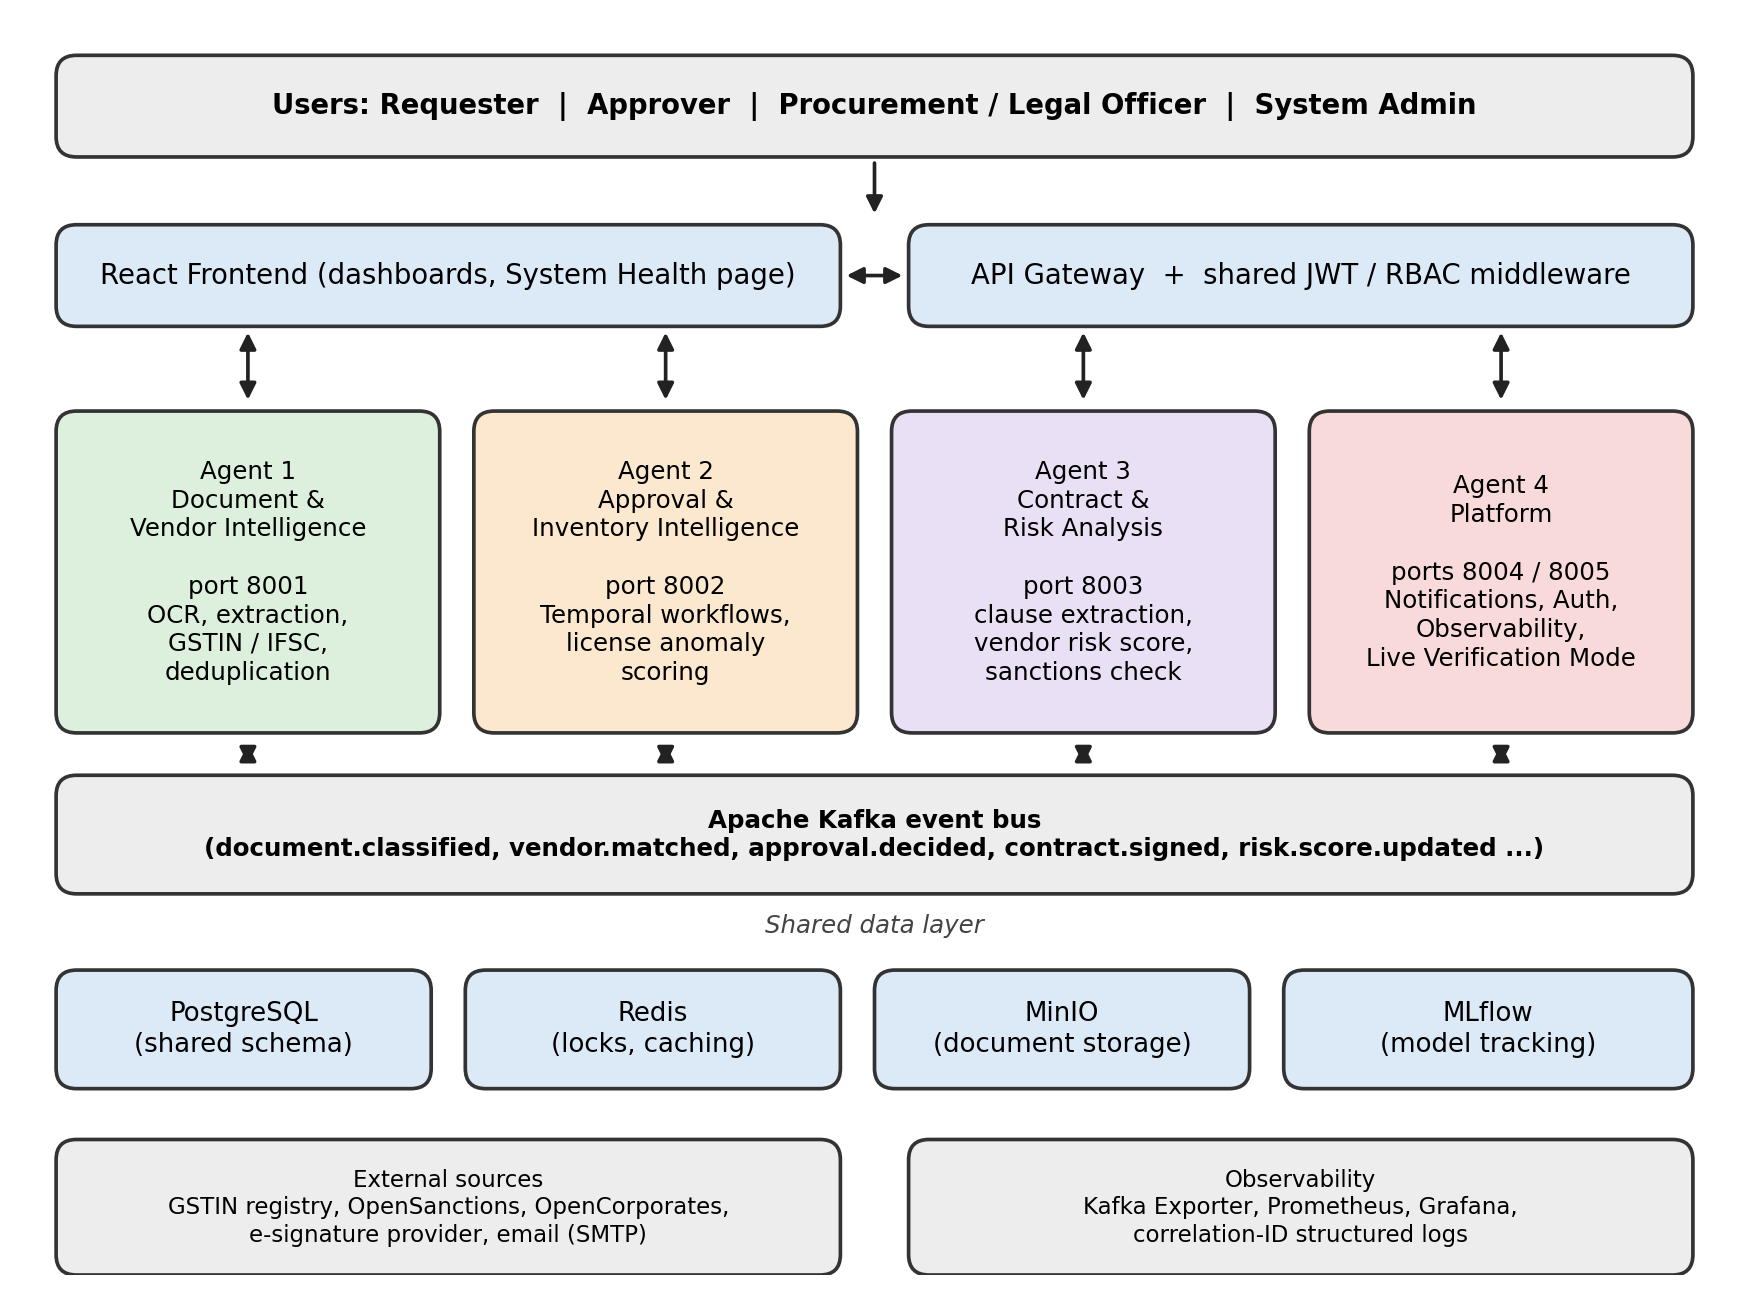
\includegraphics[width=0.92\textwidth]{figures/fig_architecture.png}
\caption{Overall architecture of the proposed system}
\label{fig:arch}
\end{figure}

Splitting the system this way keeps each concern separate. A change to the extraction models does not touch the approval engine, and a slow external lookup cannot block a user's upload, because the heavy work runs asynchronously off the request path.

\subsection{The Four Agents}

Table~\ref{tab:agents} summarises the agents, and the paragraphs that follow describe what each one does.

\begin{table}[!htbp]
\centering
\footnotesize
\renewcommand{\arraystretch}{1.2}
\caption{Summary of the four agents in the proposed system}
\label{tab:agents}
\begin{tabular}{|p{\dimexpr 0.20\textwidth-2\tabcolsep\relax}|p{\dimexpr 0.09\textwidth-2\tabcolsep\relax}|p{\dimexpr 0.35\textwidth-2\tabcolsep\relax}|p{\dimexpr 0.32\textwidth-2\tabcolsep\relax}|}
\hline
\raggedright \textbf{Agent} & \raggedright \textbf{Port} & \raggedright \textbf{Main responsibility} & \raggedright \textbf{Key techniques} \tabularnewline \hline
\raggedright Document and Vendor Intelligence & \raggedright 8001 & \raggedright Document intake, extraction, vendor identity verification, duplicate detection & \raggedright Docling, PaddleOCR, LayoutLMv3 fallback, TF-IDF classifier, rapidfuzz, ClamAV \tabularnewline \hline
\raggedright Approval and Inventory Intelligence & \raggedright 8002 & \raggedright Approval routing, SLA escalation, inventory reservation, license reclaim & \raggedright Temporal, Redis locks, Isolation Forest, SHAP \tabularnewline \hline
\raggedright Contract and Risk Analysis & \raggedright 8003 & \raggedright Contract generation, e-signature, clause extraction, vendor risk scoring, sanctions screening & \raggedright Jinja2, Legal-BERT (CUAD), FinBERT, scikit-learn, PSI drift monitoring \tabularnewline \hline
\raggedright Platform (Notifications, Auth, Observability) & \raggedright 8004 / 8005 & \raggedright Authentication and RBAC, notifications, monitoring, quota control & \raggedright JWT, Kafka consumers, Prometheus, Grafana, Live Verification Mode \tabularnewline \hline
\end{tabular}
\end{table}

\paragraph{Document and Vendor Intelligence.} This agent is the entry point for every document. It scans each upload for malware, extracts structured data, and gives each field a confidence score so that doubtful values go to a human instead of being filled in automatically. It also verifies the vendor's GSTIN and bank details, detects duplicate vendors and duplicate invoices, and never applies a change of payment details directly. Such a change waits in a pending state until a second, different user confirms it.

\paragraph{Approval and Inventory Intelligence.} This agent builds the approval chain for each request from configurable spend and budget rules, excludes the requester from their own chain, and uses Temporal to run SLA timers and escalate automatically when an approver does not respond. It reserves stock and license seats with locks so that two concurrent requests cannot take the last unit. A daily job scores license usage with an Isolation Forest model. When a license looks abandoned, the actual user is told and given seven days to object before it is reclaimed.

\paragraph{Contract and Risk Analysis.} Once a request is approved, this agent fills a contract template, sends it for e-signature and verifies the signing webhook. A question-answering model reads the contract text to pull out the renewal type, notice period and end date, so that reminders can be sent in time. The same agent keeps a running risk score for every vendor from real external sources. Facts such as a sanctions match or a cancelled GSTIN force a High rating, and only the softer signals pass through the learned model.

\paragraph{Platform.} The fourth agent handles what no single functional agent should own: authentication and access control, notification delivery, system monitoring and quota control for scarce external APIs. It also provides the correlation ID that lets one request be followed across all services.

\subsection{Document Processing Pipeline}

The most involved part of the system is the pipeline that turns an uploaded file into a trustworthy structured record, shown in Figure~\ref{fig:pipeline}. The upload returns immediately, and a Kafka consumer runs the stages in the background.

\begin{figure}[!htbp]
\centering
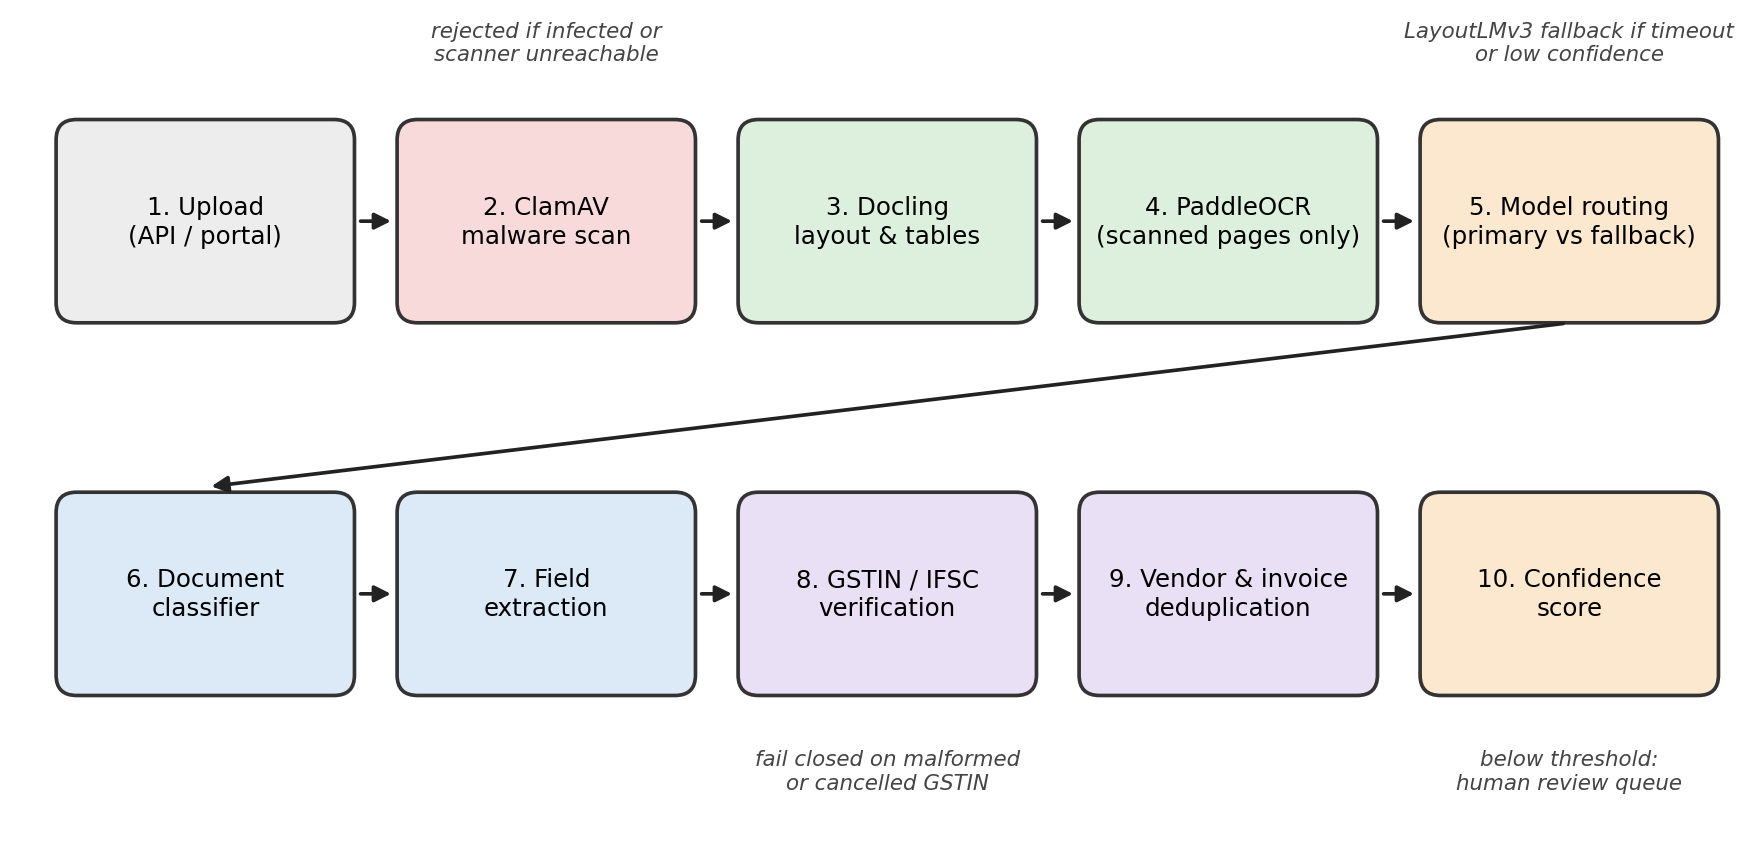
\includegraphics[width=\textwidth]{figures/fig_doc_pipeline.png}
\caption{Document processing pipeline of the Document and Vendor Intelligence agent}
\label{fig:pipeline}
\end{figure}

A file is first streamed through ClamAV and rejected if it is flagged or if the scanner cannot be reached, so the system fails closed. Docling then recovers layout and tables, and PaddleOCR is used only for pages without a text layer. If the primary pipeline times out or its confidence is low, LayoutLMv3 runs as an independent fallback. A trained classifier labels the document as a purchase order, invoice or quote, and the extracted fields are written into the shared schema. The vendor's GSTIN is checked next, and the vendor is matched against existing records, with the GSTIN taking priority over name similarity. Finally, each field receives a confidence score, and anything below the threshold is placed in the review queue.

\subsection{Inter-Agent Communication and Workflow}

Figure~\ref{fig:events} shows how the agents exchange events, and Table~\ref{tab:events} lists the main ones. A single correlation identifier is created at the start of a business flow and carried unchanged through every event and log line, so the full journey of one document or request can be traced.

\begin{figure}[!htbp]
\centering
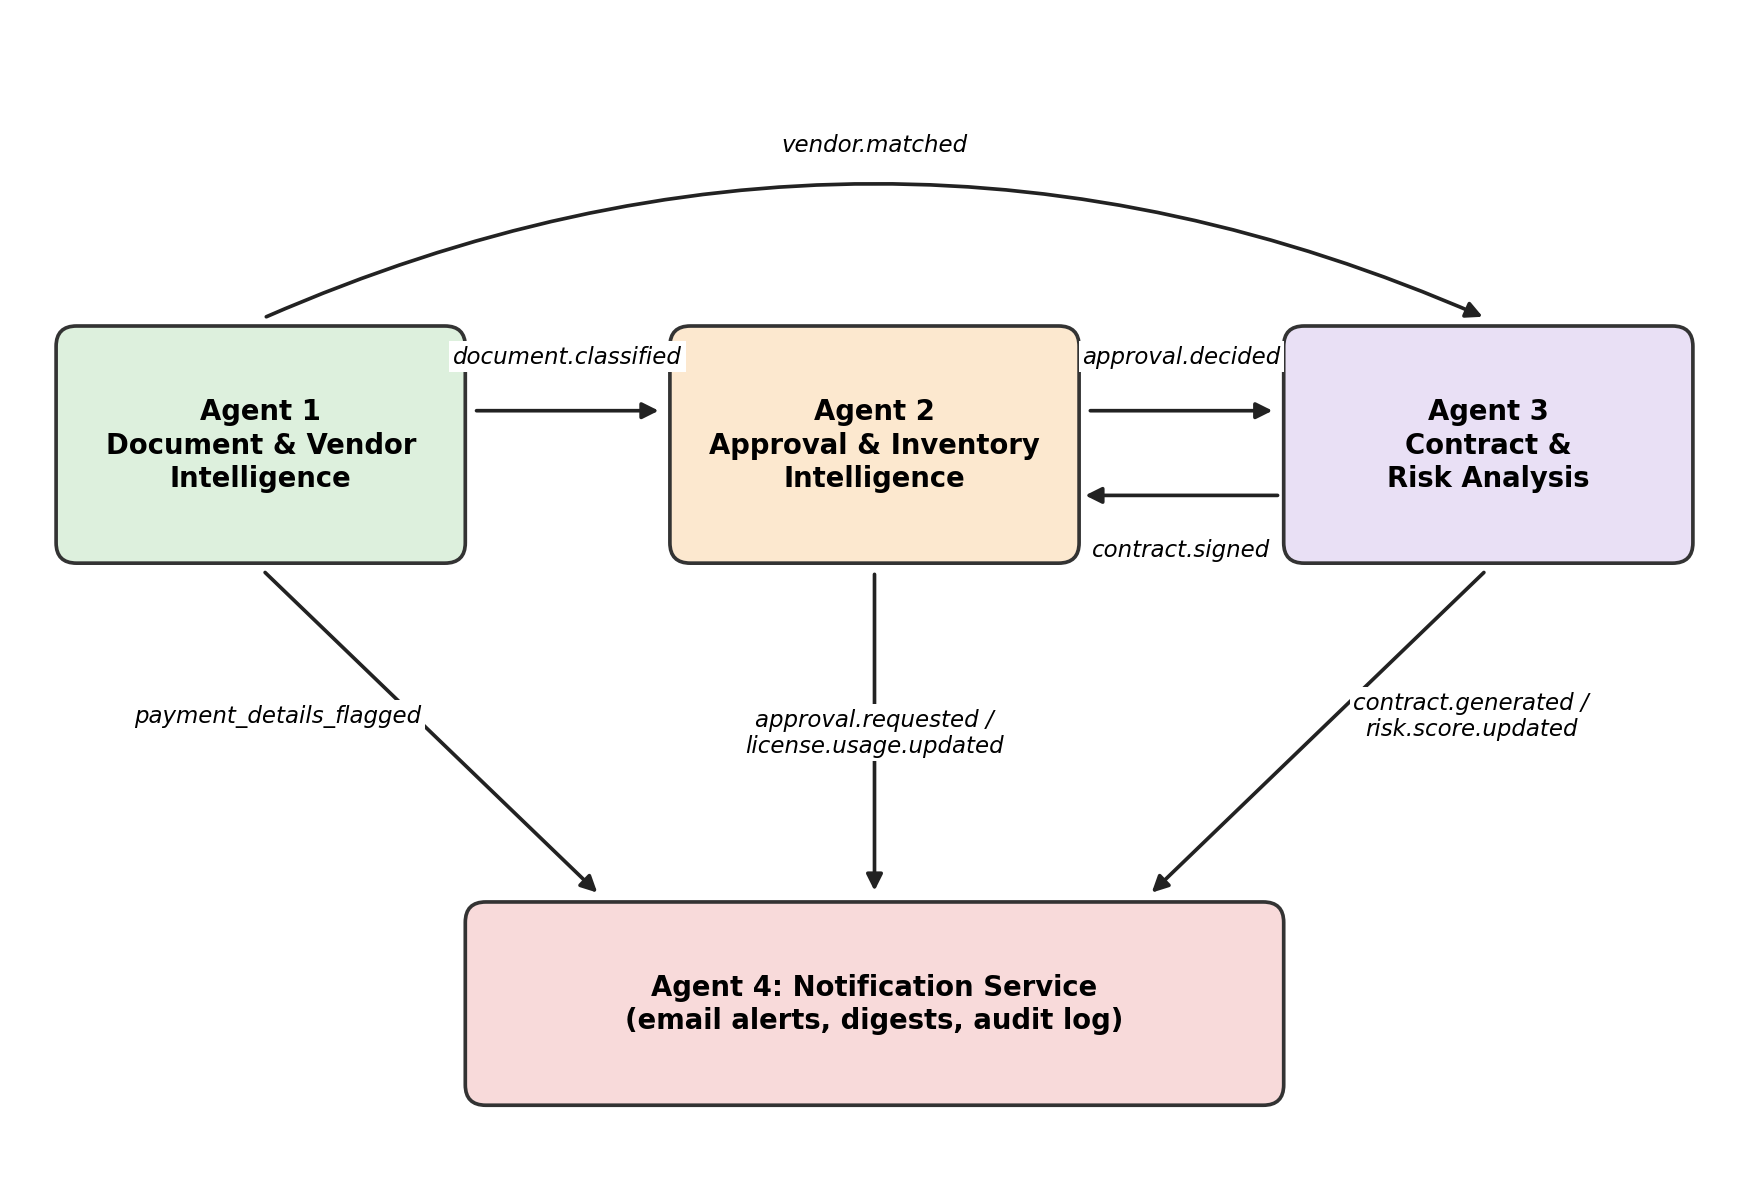
\includegraphics[width=0.9\textwidth]{figures/fig_event_flow.png}
\caption{Event flow between the agents}
\label{fig:events}
\end{figure}

\begin{table}[!htbp]
\centering
\footnotesize
\renewcommand{\arraystretch}{1.2}
\caption{Main events exchanged between agents}
\label{tab:events}
\begin{tabular}{|p{\dimexpr 0.29\textwidth-2\tabcolsep\relax}|p{\dimexpr 0.24\textwidth-2\tabcolsep\relax}|p{\dimexpr 0.43\textwidth-2\tabcolsep\relax}|}
\hline
\raggedright \textbf{Event} & \raggedright \textbf{Published by} & \raggedright \textbf{Consumed by and purpose} \tabularnewline \hline
\raggedright document.classified & \raggedright Agent 1 & \raggedright Agent 2 and notifications: structured extraction result \tabularnewline \hline
\raggedright vendor.matched & \raggedright Agent 1 & \raggedright Agent 3: verified vendor identity for risk scoring \tabularnewline \hline
\raggedright vendor.payment\_\allowbreak details\_\allowbreak flagged & \raggedright Agent 1 & \raggedright Notifications: immediate finance alert on a payment-detail change \tabularnewline \hline
\raggedright approval.requested / approval.decided & \raggedright Agent 2 & \raggedright Agent 3 and notifications: drives contract generation and alerts \tabularnewline \hline
\raggedright license.usage.updated & \raggedright Agent 2 & \raggedright Notifications: utilisation and anomaly alerts \tabularnewline \hline
\raggedright contract.generated / contract.signed & \raggedright Agent 3 & \raggedright Agent 2 and notifications: fulfilment closure \tabularnewline \hline
\raggedright contract.renewal.due & \raggedright Agent 3 & \raggedright Notifications: 60, 30 and 15 day renewal reminders \tabularnewline \hline
\raggedright risk.score.updated & \raggedright Agent 3 & \raggedright Notifications: high-risk alerts \tabularnewline \hline
\end{tabular}
\end{table}

{\sloppy In a typical run, a requester uploads a document and Agent~1 publishes \texttt{document.classified} together with \texttt{vendor.matched}. Agent~2 builds the approval chain and, once the final approver agrees, publishes \texttt{approval.decided}. Agent~3 then generates the contract and sends it for signature, and its \texttt{contract.signed} event tells Agent~2 to mark the request as fulfilled and activate the asset. The notification agent listens to all of these events and sends urgent alerts, such as a flagged payment-detail change, immediately while batching routine ones.\par}

\subsection{Use Case View}

Figure~\ref{fig:usecase} presents the use case diagram of the system. Four actors take part: the System Admin, who configures business rules; the Requester, who submits purchase requests; the Approver, who approves or rejects them; and the Procurement or Legal Officer, who handles vendor documents and contracts. The use cases are grouped into five phases.

\begin{figure}[!htbp]
\centering
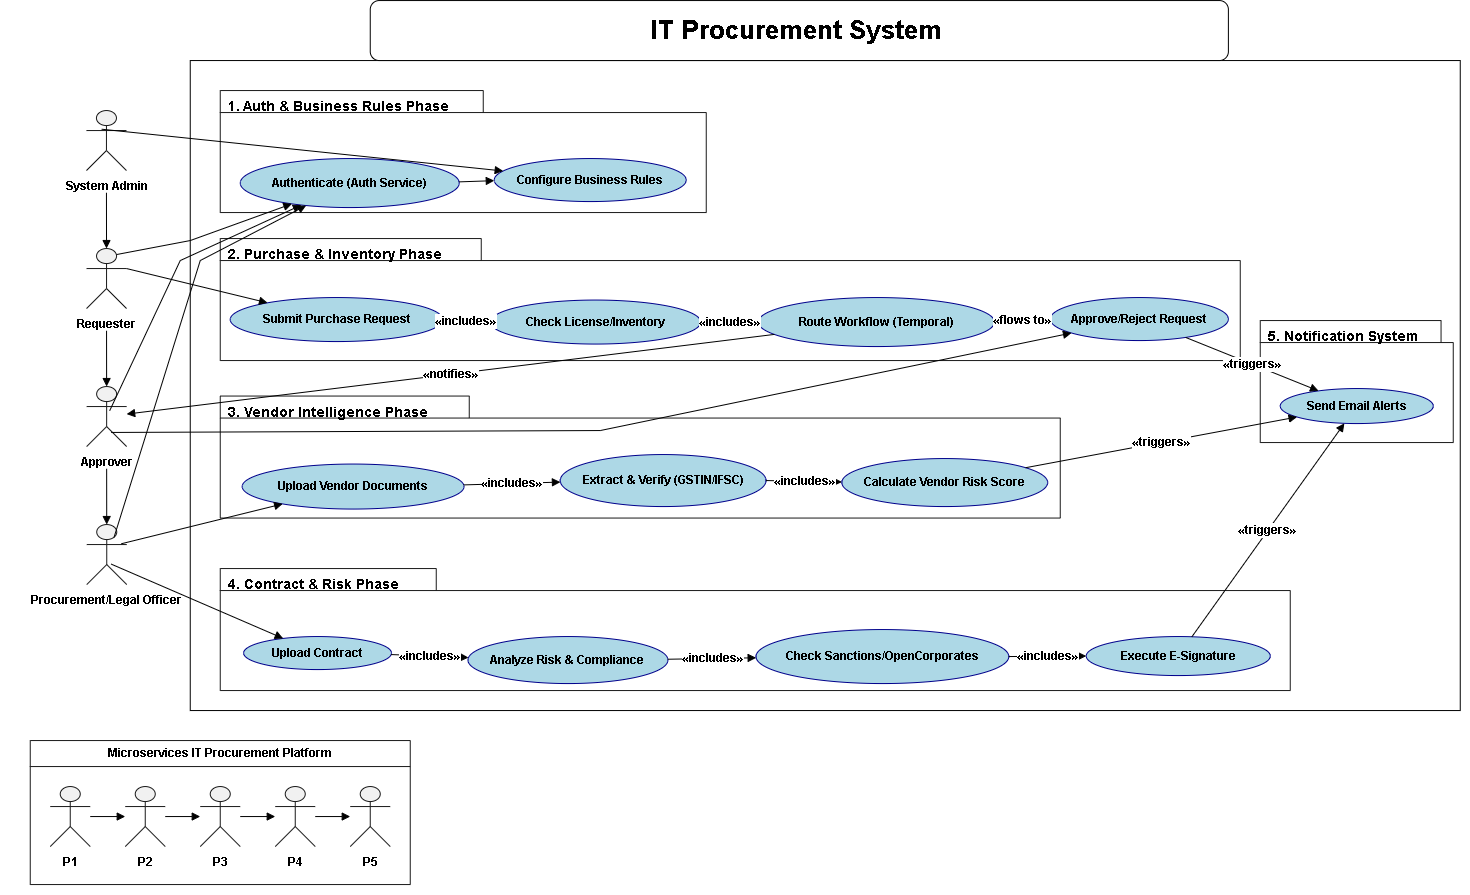
\includegraphics[width=\textwidth]{figures/usecase.png}
\caption{Use case diagram of the IT procurement system}
\label{fig:usecase}
\end{figure}

\begin{enumerate}
\item \textbf{Authentication and business rules.} Users sign in through the authentication service, and the administrator configures the business rules that drive routing.
\item \textbf{Purchase and inventory.} A requester submits a purchase request, the system checks license and inventory availability, the approval workflow is routed through Temporal, and the approver approves or rejects.
\item \textbf{Vendor intelligence.} Vendor documents are uploaded, GSTIN and IFSC details are extracted and verified, and a vendor risk score is calculated.
\item \textbf{Contract and risk.} A contract is uploaded or generated, analysed for risk and compliance, checked against sanctions and company registry data, and finally signed electronically.
\item \textbf{Notification.} Approvals, risk scores and signature events trigger email alerts to the people concerned.
\end{enumerate}

\subsection{Technology Stack}

Table~\ref{tab:stack} lists the main technologies. Wherever possible, pretrained open-source models are used, and only the document classifier and the usage anomaly and risk models are trained within the project.

\begin{table}[!htbp]
\centering
\footnotesize
\renewcommand{\arraystretch}{1.2}
\caption{Technology stack of the proposed system}
\label{tab:stack}
\begin{tabular}{|p{\dimexpr 0.24\textwidth-2\tabcolsep\relax}|p{\dimexpr 0.38\textwidth-2\tabcolsep\relax}|p{\dimexpr 0.34\textwidth-2\tabcolsep\relax}|}
\hline
\raggedright \textbf{Layer} & \raggedright \textbf{Technology} & \raggedright \textbf{Purpose} \tabularnewline \hline
\raggedright Frontend & \raggedright React & \raggedright Dashboards and System Health page \tabularnewline \hline
\raggedright Backend services & \raggedright FastAPI (Python), Docker & \raggedright One containerised service per agent \tabularnewline \hline
\raggedright Messaging & \raggedright Apache Kafka & \raggedright Asynchronous events between agents \tabularnewline \hline
\raggedright Workflow engine & \raggedright Temporal & \raggedright Approval workflows, SLA timers, escalation \tabularnewline \hline
\raggedright Data stores & \raggedright PostgreSQL, Redis, MinIO & \raggedright Records, locks and caching, document files \tabularnewline \hline
\raggedright Document AI & \raggedright Docling, PaddleOCR, LayoutLMv3 & \raggedright Layout analysis, OCR, fallback extraction \tabularnewline \hline
\raggedright Language and risk models & \raggedright Legal-BERT, FinBERT, scikit-learn, SHAP & \raggedright Clause extraction, adverse media, risk and anomaly scoring \tabularnewline \hline
\raggedright Security & \raggedright JWT, ClamAV, Pwned Passwords check & \raggedright Authentication, malware scanning, password safety \tabularnewline \hline
\raggedright Monitoring & \raggedright MLflow, Kafka Exporter, Prometheus, Grafana & \raggedright Model tracking, consumer lag, dashboards \tabularnewline \hline
\raggedright Notifications & \raggedright Jinja2 templates, SMTP (Mailpit in development) & \raggedright Templated email alerts \tabularnewline \hline
\end{tabular}
\end{table}

\subsection{Key Design Principles}

Four principles run through the whole design. The system is \emph{fraud-aware}: uploads are scanned and rejected if the scanner is unavailable, and payment-detail changes need a second person's confirmation. It is \emph{fair}: a user gets a grace period before a license is reclaimed, and a vendor is never scored worse only because some data could not be retrieved. It is \emph{accountable}: every override or sanctions-flag clearance needs a logged justification, and the risk model is monitored for drift. Finally, it is \emph{traceable}: one correlation ID follows a request through every service, and a System Health page shows Kafka lag and recent activity.

%%%%%%%%%%%%%%%%%%%%%%%%%%%%%%%%%%%%%%%%%%%%%%%%%%%
%%% End of Chapter 3